\documentclass[11pt]{article}
\usepackage{tikz}
\usepackage{endiagram}
\usepackage{chemmacros}
\chemsetup{modules={all}}
\usetikzlibrary{automata,positioning,arrows}
\NewChemPhase\lqdd{\(\ell\)}
\NewChemPhase\gr{grafite}
\NewChemPhase\reac{reação}
\usepackage{siunitx}

\begin{document}
%%% https://vestibulares.estrategia.com/public/questoes/diagrama-entalpia-para447a186d1a/
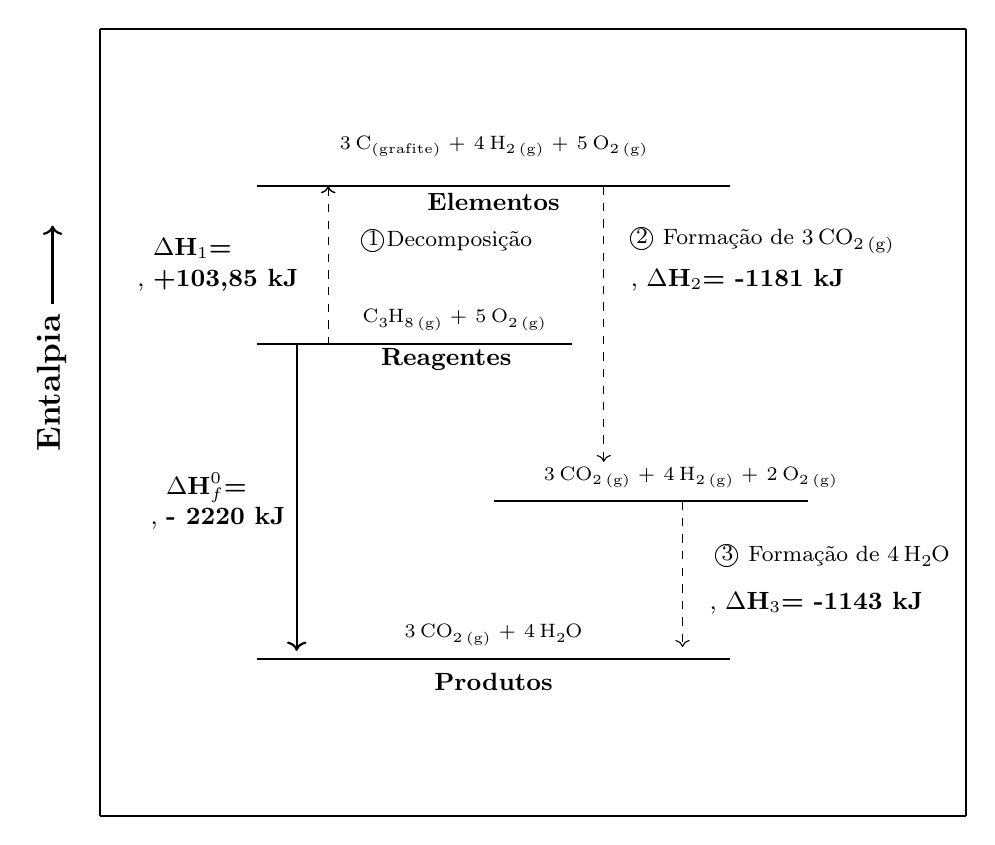
\begin{tikzpicture}
[scale=1]
\tikzstyle{every node}=[font=\scriptsize]

%\draw[step=1cm,black,very thin] (0,0) grid (10,10);
\draw[thick,-](0,0) -- (0,10); %% borda y
\draw[thick,-](11,10) -- (0,10); %% borda em top
\draw[thick,-](0,0) -- (11,0); %% borda  X
\draw[thick,-](11,0) -- (11,10); %% Eixo y2
%%%%  Line 
\draw[thick,-](2,8) -- (8,8);
\draw(5,8.5) node{\ch{3 C_{(grafite)} + 4 H2_{\gas} + 5 O2_{\gas}}};
\draw(5,7.8) node{\small \bfseries Elementos};
\draw[dashed,<-](2.9,8)--(2.9,6.0);
\draw(4.4,7.3) node[font={\footnotesize}]{\textcircled{1}Decomposição};
\draw(1.5,7) node[align=left, font={\small, \bfseries}]{$\Delta$H$_1$=\\ +103,85 kJ};
%%%% 
%%%% Line 2
\draw[thick,-](2,6) -- (6,6);
\draw(4.5,6.3) node{\ch{C3H8_{\gas} + 5 O2_{\gas}}};
\draw(4.4,5.8) node{\small \bfseries Reagentes};
\draw(8.4,7.3) node[font={\footnotesize}]{\textcircled{2} Formação de \ch{3 CO2_{\gas}}};
\draw(8.1,6.8) node[align=left, font={\small, \bfseries}]{$\Delta$H$_2$= -1181 kJ};
\draw[dashed,<-](2.9,8)--(2.9,6.0);
%%%% Line 3
\draw[thick,-](5,4) -- (9,4);
\draw(1.5,4) node[align=left, font={\small, \bfseries}]{$\Delta$H$^0_f$=\\ - 2220 kJ};
\draw[dashed,->](6.4,8)--(6.4,4.5);
\draw(7.5,4.3) node{\ch{3 CO2_{\gas} + 4 H2_{\gas} + 2 O2_{\gas}}};
%%%% Line 4
\draw[thick,-](2,2) -- (8,2);
\draw(5,1.7) node{\small \bfseries Produtos};
\draw(5,2.3) node{\ch{3 CO2_{\gas} + 4 H2O_{\lqdd}}};
\draw[thick,->](2.5,6)--(2.5,2.1);
\draw(9.3,3.3) node[font={\footnotesize}]{\textcircled{3} Formação de \ch{4 H2O}};
\draw[dashed,->](7.4,4)--(7.4,2.15);
\draw(9.1,2.7) node[align=left, font={\small, \bfseries}]{$\Delta$H$_3$= -1143 kJ};
%%%% Seta Eixo
\draw(-.3,5.5) node[sloped,anchor=center, rotate=90, above]{\large \bfseries Entalpia};
\draw[thick,->](-.6,6.5)--(-.6,7.5);

\end{tikzpicture}

\newpage 


\begin{endiagram}[
tikz         = {xscale=2.5}, scale        = 0.8,
%y-label-offset=25pt,
y-label-text = Entalpia (kJ/mol),
energy-step=50,
%energy-zero=-200=
%energy-unit=\kilo\joule\per\mole,
x-label      = below,        x-label-text = progresso da reação,]
\ENcurve{11,11,14,8,8}
%\AddAxisLabel{(N1-1)[0];(N1-4)[-225];(N1-3)[560]}
\ShowNiveaus[niveau=N1-1,shift=-0.5]
\ShowNiveaus[niveau=N1-4,shift=.5]
\draw[above left] (N1-1) ++ (2,1) node {\small \ch{CO_{\gas} + NO2_{\gas}}} ;
\draw[above] (N1-4) ++ (.8,0) node {\small\ch{CO2{\gas} + NO_{\gas}} } ;
\end{endiagram}

\newpage

\begin{endiagram}[
tikz         = {xscale=2.5}, scale        = 0.8,
y-label-offset=25pt,
y-label-text = Entalpia (kJ/mol),
x-label      = below,        x-label-text = progresso da reação,]
\ENcurve{1,1,11,5,5}
\AddAxisLabel{(N1-1)[0];(N1-4)[226];(N1-3)[560]}
\ShowNiveaus[niveau=N1-1,shift=-0.5]
\ShowNiveaus[niveau=N1-4,shift=.5]
\draw[above left] (N1-1) ++ (2,1) node {\small \ch{2 C_{(grafite)} + H2_{\gas}}} ;
\draw[above] (N1-4) ++ (.8,0) node {\small\ch{C2H2_{\gas}} } ;
\end{endiagram}




\newpage 




\begin{endiagram}[
tikz         = {xscale=2.5}, scale        = 0.8,
y-label-offset=25pt,
y-label-text = Entalpia (kJ/mol),
x-label      = below,        x-label-text = progresso da reação,]
\ENcurve{5,8,0,0}
\AddAxisLabel{(N1-1)[965];(N1-2)[1215];(N1-3)[75]}
\ShowNiveaus[niveau=N1-1,shift=-0.5]
\ShowNiveaus[niveau=N1-3,shift=.5]
\draw[above left] (N1-1) ++ (0.6,1) node {\small \ch{CH4 + 2 O2} } ;
\draw[above] (N1-3) ++ (.8,0) node {\small\ch{CO2 + 2 H2O} } ;
\end{endiagram}





\newpage 

 

\newpage

\begin{reactions*}
CaCO3_{\sld} -> CO2_{\gas} + CaO_{\sld} & $\qquad \enthalpy{178}$ \\
CaO_{\sld}   
\end{reactions*}

Observe o diagrama a seguir
\begin{center}
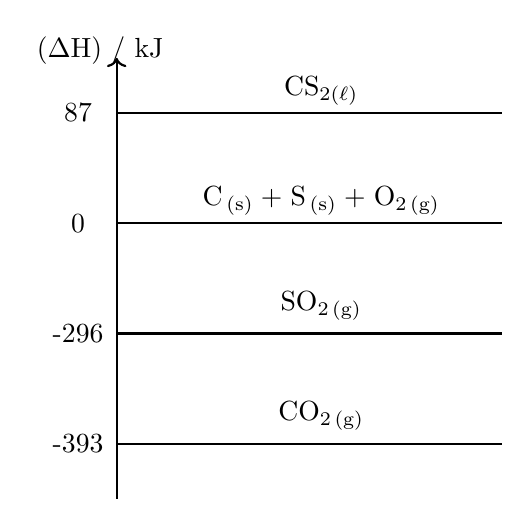
\begin{tikzpicture}[scale=.7]
\draw[thick,->](0,0) -- (0,8);
\draw(-.3,7.7) node[sloped,anchor=center, rotate=0, above]{($\Delta$H) / kJ};
%Line 1
\draw[thick,-](0,7) -- (7,7);
\draw(-0.7,7) node{87};
\draw(3.7,7.4) node{\ch{CS2_{($\ell$)}}};
%% Line 2
\draw[thick,-](0,5) -- (7,5);
\draw(-0.7,5) node{0};
\draw(3.7,5.4) node{\ch{C_{\sld} + S_{\sld} + O2_{\gas}}};
%%% Line 3
\draw[thick,-](0,3) -- (7,3);
\draw(-0.7,3) node{-296};
\draw(3.7,3.5) node{\ch{SO2_{\gas}}};
%%%%% Line 4
\draw[thick,-](0,1) -- (7,1);
\draw(-0.7,1) node{-393};
\draw(3.7,1.5) node{\ch{CO2_{\gas}}};
\end{tikzpicture}
\end{center}
Qual o valor da entalpia da reação para a reação a seguir.
\begin{reaction*}
CS2_{\lqd} + 3 O2_{\gas} -> CO2_{\gas} + 2 SO2_{\gas}
\end{reaction*}

\newpage


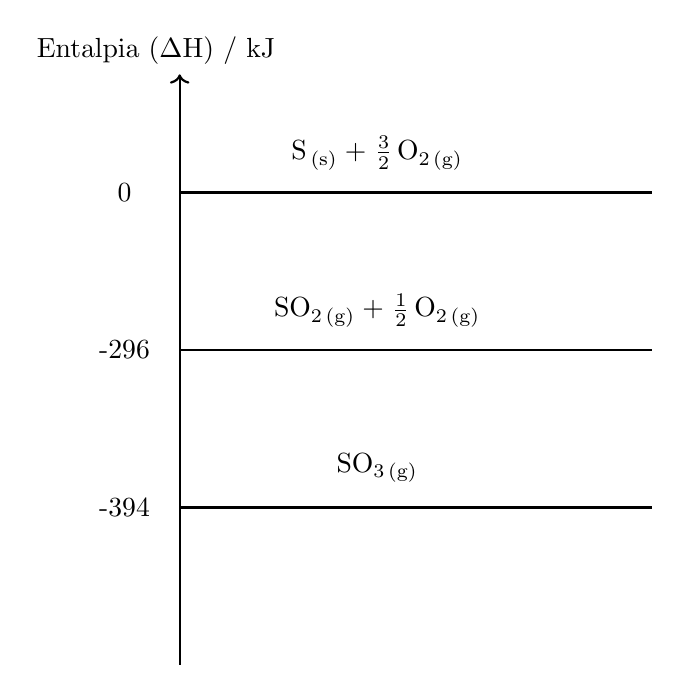
\begin{tikzpicture}[scale=1]
%\draw[step=1cm,black,very thin] (0,0) grid (10,10);
\draw[thick,->](0,0) -- (0,7.5);
\draw(-.3,7.5) node[sloped,anchor=center, rotate=0, above]{Entalpia ($\Delta$H) / kJ};
%% Line 1
\draw[thick,-](0,2) -- (6,2);
\draw(-0.7,2) node{-394};
\draw(2.5,2.5) node{\ch{SO3_{\gas}}};
%%% Line 2
\draw[thick,-](0,4) -- (6,4);
\draw(-0.7,4) node{-296};
\draw(2.5,4.5) node{\ch{SO2_{\gas} + 1/2 O2_{\gas}}};
%%% Line 3
\draw[thick,-](0,6) -- (6,6);
\draw(-0.7,6) node{0};
\draw(2.5,6.5) node{\ch{S_{\sld} + 3/2 O2_{\gas}}};
\end{tikzpicture}
\newpage






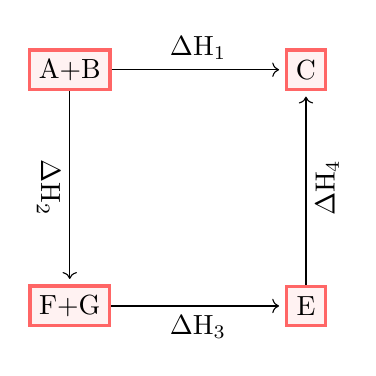
\begin{tikzpicture}[
squarednode/.style={rectangle, draw=red!60, fill=red!5, very thick, minimum size=5mm}, shorten >=2pt,node distance=3cm,on grid,
]
\node[squarednode] (1) {A+B};
\node[squarednode] (2) [right=of 1] {C};
\node[squarednode] (3) [below=of 1] {F+G};
\node[squarednode] (4) [right= of 3] {E};
%%% 
%% Lines
\draw[->] (1.east) -- node[above]{$\Delta$H$_1$}(2.west);
\draw[->] (1.south) -- node[sloped, anchor=center, below]{$\Delta$H$_2$}(3.north);
\draw[->] (3.east) -- node[below]{$\Delta$H$_3$}(4.west);
\draw[->] (4.north) -- node[sloped, anchor=center, below]{$\Delta$H$_4$}(2.south);
\end{tikzpicture}



\begin{endiagram}[
x-label=right,
y-label= above, y-label-text = Energia,
x-label= below, x-label-text = Progresso da Reação]
\ENcurve{4,4,4,-1,-1,-1}
\end{endiagram}


$\Delta$H$_1$ + $\Delta$H$_2$ + $\Delta$H$_4$


\end{document}

